\chapter{問題與討論}
 Q:我們執行sample.py時,python出現了print錯誤。(如:圖8.1)\\
\begin{figure}[hbt!]
\begin{center}
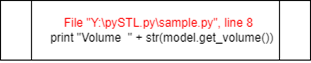
\includegraphics[width=15cm]{print錯誤}
\caption{\Large print錯誤}
\label{print錯誤}
\end{center}
\end{figure}

A:我們必須把sample.py與pySTL.py裡的全部的print加上括號,才能避免上述狀況的發生。(如:圖8.2)\\

\begin{figure}[hbt!]
\begin{center}
\includegraphics[width=15cm]{print加()}
\caption{\Large print加()}
\label{print加()}
\end{center}
\end{figure}

Q:再次執行sample.py時,pySTL.py出現語法錯誤。(圖.\ref{self.centroid==None語法錯誤})。\\
\begin{figure}[hbt!]
\begin{center}
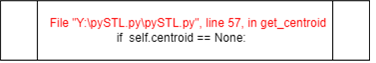
\includegraphics[width=15cm]{self.centroid==None語法錯誤}
\caption{\Large self.centroid==None語法錯誤}
\label{self.centroid==None語法錯誤}
\end{center}
\end{figure}
\qquad \\
A:透過網路的搜尋,找到將==改成is,才可以與None進行比較,所以我們把pySTL裡的line57與line62的==改成is。(如:圖8.4):\\

\begin{figure}[hbt!]
\begin{center}
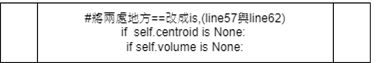
\includegraphics[width=10cm]{將==改成is}
\caption{\Large 將==改成is}
\label{將==改成is}
\end{center}
\end{figure}
%\fontsize{0.001pt}{1pt}\selectfont .\\ %圖片間距勿刪

Q:再次執行sample.py時,pySTL.py出現語法錯誤。(如:圖8.3)。\\
\begin{figure}[hbt!]
\begin{center}
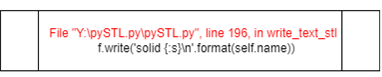
\includegraphics[width=15cm]{self.name錯誤}
\caption{\Large self.name錯誤}
\label{self.name錯誤}
\end{center}
\end{figure}
\qquad \\


A:仔細讀了pySTL裡line196上下的代碼,發現到這段的語法是要開啟ASCII的STL檔案,所以不能使用二進位(wb)的方式來寫入檔案,所以把wb改成w,即可排除上述的錯誤。(如:圖8.4)\\
\begin{figure}[hbt!]
\begin{center}
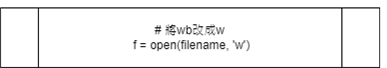
\includegraphics[width=15cm]{將w改成wb}
\caption{\Large 將w改成wb}
\label{將w改成wb}
\end{center}
\end{figure}


Q:再次執行sample.py時,雖然python沒有顯示錯誤,但是寫出的stl檔案格式無法開啟。\\

A:仔細讀了pySTL代碼,發現到line99是使用’rb’來讀取檔案,但是line104裡,沒有使用位元(b)讀取檔案,導致判斷ASCII stl 都會變成binary stl,導致計算ASCII尺寸錯誤無法順利開啟檔案,所以改成b’solid’即可修正問題。(如:圖8.5)\\
\begin{figure}[hbt!]
\begin{center}
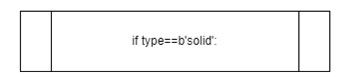
\includegraphics[width=15cm]{type==b'solid'}
\caption{\Large type==b'solid'}
\label{type==b'solid'}
\end{center}
\end{figure}
